\documentclass[12pt,a4paper]{article}
\usepackage[spanish]{babel}
\usepackage[utf8]{inputenc}
\usepackage{graphicx}
\usepackage{graphics}
\usepackage{epsfig}
\usepackage{amsmath}
\usepackage{algorithm}
\usepackage{algorithmic}
\usepackage{url,hyperref,times}
\usepackage[T1]{fontenc}
\usepackage{color,listings,tikz}
\selectlanguage{spanish}
\usepackage{times}
\usepackage{verbatim,scalefnt,colortbl}
\newtheorem{mydef}{Definición}
\providecommand{\e}[1]{\ensuremath{\times 10^{#1}}}

\title{ {\bf Whole genome alignment in high performance computing environments} \\
\it Informe del progreso de trabajo de investigaci\'on} 
\author{ {\bf Julio C\'esar Garc\'ia Vizca\'ino}  \\ 
Departamento de Arquitectura de Computadores y Sistemas Operativos \\ 
Universidad Aut\'onoma de Barcelona\\ 
{\small jcgarcia@aomail.uab.es} 
}
\date{\today}

\begin{document}
\pagestyle{plain}
\pagenumbering{roman}
\maketitle
\pagebreak
{\Huge{\bf Datos del doctorando}}\\
{\Large \\Nombre Completo: Julio Csar García Vizcaíno\\}
\vspace{0.3cm}
{\Large NIE: Y1497678R\\}
{\Huge{\bf Datos del proyecto de tesis}}\\
\vspace{0.3cm}
{\Large \\Estudio de doctorado: Computación de Altas Prestaciones\\}
\vspace{0.3cm}
{\Large \\Título del proyecto de tesis doctoral: \emph{
Whole genome alignment in high performance computing environments.}\\}
\vspace{0.3cm}
%{\Large \\Palabras claves: Alineamiento de genoma, cadena coincidente,
%datos de secuencia biol\'ogica a gran escala, C\'omputo de altas prestaciones.\\}
%\vspace{0.5cm}
{\Large \\Directores de la tesis: Antonio Espinosa, Juan Carlos Moure.\\}
\vspace{0.3cm}
{\Large \\Línea de investigación: Aplicaciones bioinformáticas.\\}
\vspace{0.3cm}
{\Large \\Rgimen de dedicación: completa.\\}
\vspace{0.3cm}
{\Large \\A\~no de inscripci\'on: 2011.\\}
\vspace{0.3cm}
{\Large \\A\~no previsto para la presentaci\'on de Tesis Doctoral: 2014\\}
\vspace{0.3cm}
{\large \\Firmado\\}
\vspace{2.8cm}
\begin{center}
\begin{tabular}{ c c c }
Director & Director & Estudiante\\
Antonio Espinos & Juan Carlos Moure & Julio C\'esar García Vizcaíno\\
\end{tabular}
\end{center}
\pagebreak
%\cleardoublepage
\pagenumbering{arabic}
\section{Resumen}
\indent
Actualmente la generación de nueva información genómica ha creado la necesidad de almacenar y procesar estos nuevos datos computacionalmente hablando. Una de las tareas en la que nos centramos es en el alineamiento de genomas. La información básica de un genoma es el ADN. El ADN es una cadena compuesta por el alfabeto $\sigma={a,c,g,t}$, cada uno de estos elementos es llamado nucleótido. El alineamiento de genomas consiste en encontrar las similitudes y diferencias de las cadenas de ADN entre genomas.\\
El alineamiento de genomas es un modelo matemático utilizado por los biólogos para determinar la similitud entre genomas. Un alineamiento involucra tres operaciones básicas:
\begin{itemize}
  \item Coincidencia: los nucleótidos en ambos genomas son iguales.
  \item Discrepancia: los nucleótidos no coinciden en ambos genomas.
  \item Mutaciones: uno o varios cambios de nucleótidos en el genoma:
    \begin{itemize}
      \item Sustitución: un nucleótido es reemplazado por otro.
      \item Inserción: uno o varios nucleótidos se insertan en una posición en el genoma.
      \item Eliminación: uno o varios nucleótidos se borran del genoma.
    \end{itemize}
\end{itemize}
Los algoritmos utilizados para el alineamiento de genomas presentan una alta demanda computacional debido al tamaño de los datos genómicos.\\
\indent
Existe diferentes algoritmos propuestos para el alineamiento de dos secuencias como \cite{Needleman1970General} y \cite{Waterman}. Estos algoritmos funcionan bien con tamaños de secuencias pequeños como un gen, 20-30kbp\footnote{bp es la únidad básica de medida en las secuencias de ADN y representa la longitud de un nucleótido}. Sin embargo, son ineficaces al alinear genomas enteros. La complejidad computacional y espacial es $O(nm)$, donde $n$ y $m$ son las longitudes de los genomas a alinear. Estos algoritmos tienen problemas de mayores requerimientos de memoria o de tiempos de ejecución inaceptables.\\
\indent
Para grandes secuencias, como el genoma humano (3Gbp), el uso de recursos computacionales pueden ser extremadamente grande y con un largo tiempo de ejecución. Es por ello que han surgido alternativas para reducir el tiempo de ejecución del alineamiento de secuencias. Una de esas alternativas es la utilización de la heurística basada en las coincidencias exactas máximas en las secuencias a alinear. Al encontrar las coincidencias exactas máximas se puede realizar el alineamiento de genomas enteros reduciendo el espacio del alineamiento a las regiones entre las coincidencias exactas máximas.\\
\indent
Formalmente el problema de la búsqueda de coincidencias exactas máximas se define como:
\begin{mydef}
  Dadas dos secuencias (genomas) $R=r_{1}r_{2}\hdots r_{n}$ y $Q=q_{1}q_{2}\hdots q_{m}$, y una longitud mínima $l$, se requiere encontrar todas las ocurrencias de las coincidencias exactas máximas de longitud mínima $l$, entre $R$ y $Q$.
\end{mydef}
Existen diferentes aproximaciones para resolver el problema ver Figura \ref{fig:state}, todas ellas involucran un sacrificio de recursos de cómputo (memoria, procesador).
\begin{figure}[h] 
   \centering 
   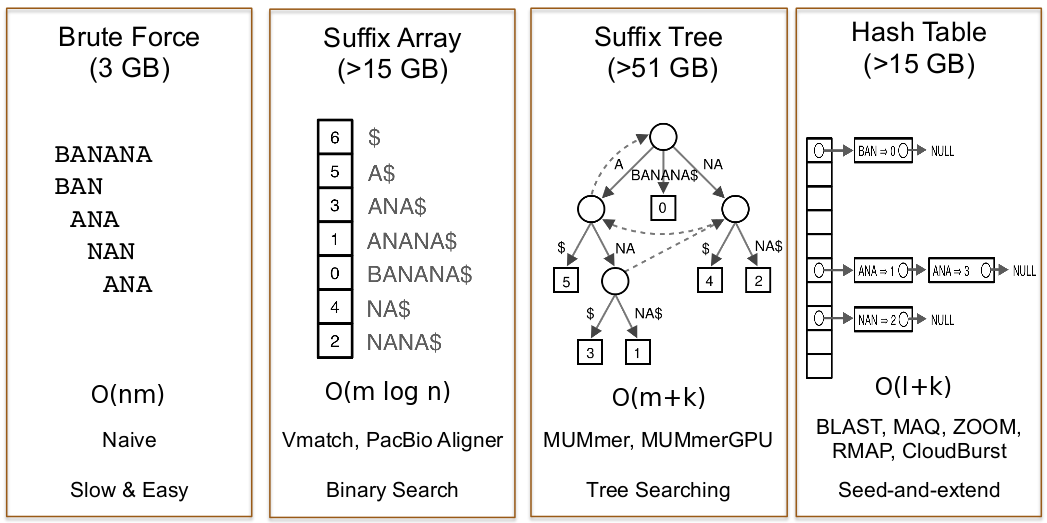
\includegraphics[scale=0.3]{state.png} 
   \caption{Diferentes soluciones al problema de la búsqueda de coincidencias exactas máximas para el genoma humano como referencia.} 
   \label{fig:state} 
 \end{figure}
\indent
El árbol de sufijos es una estructura de datos que permite la b\'usqueda de 
coincidencias exactas de longitud variable en tiempo lineal. Una coincidencia exacta de longitud $w$ ocurre en $r_{i}r_{i+1}\hdots r_{i+l-1}$ y $q_{j}q_{j+1}\hdots q_{j+l-1}$ si y solo si los sufijos $r_{i}r_{i+1}\hdots r_{n}$ y $q_{j}q_{j+1}\hdots q_{m}$ comparten un prefijo común de longitud mínima $l$. La búsqueda de coincidencias máximas exactas en un árbol de sufijos se realiza recorriendo el trayecto que es común a la secuencia de consulta hasta encontrar una discrepancia. Si la búsqueda termina en un nodo hoja, la coincidencia es única en la secuencia de referencia. Verificando el carácter inmediato anterior al inicio de esta coincidencia se puede determinar si es una coincidencia  máxima.\\
\indent
Sin embargo los requerimientos de espacio necesario para almacenar el \'arbol de sufijos en 
memoria principal la hacen una estructura inviable cuando el \'arbol de sufijos a
almacenar supera la memoria disponible.\\
\indent
Este problema se presenta en aplicaciones de alineamiento de genomas donde el
tama\~no de los genomas son de millones de caracteres y su representación en un
árbol de sufijos se hace inviable si no se tiene la cantidad de memoria 
disponible. Además, la razón de utilizar un árbol de sufijos radica en
que la búsqueda de coincidencias exactas de longitud variable en un árbol de 
sufijos se realiza en tiempo lineal, gracias al uso de los enlaces de sufijos.\\
\indent
En consecuencia se busca \textbf{acelerar la búsqueda eficiente de 
coincidencias exactas y que tenga en cuenta el uso de recursos de cómputo y
memoria}. Las consideraciones que se toman en cuenta son la longitud del genoma 
de referencia (sobre la que se realiza la búsqueda), del genoma de consulta y la longitud de la 
coincidencia a buscar.
\section{Introducción} 
\subsection{MUM y MEM} 
\indent
La heurística basada en la búsqueda de coincidencias exactas máximas para el alineamiento de genomas requiere de la definición formal de una coincidencia exacta máxima (MEM).\\
\begin{mydef}
  Un MEM (Maximal Exact Match) es una subcadena común a dos
  genomas que es mayor que una longitud mínima específica $d$ de tal manera
  que es máxima, esto es, que no puede ser extendida en ambos extremos sin
  incurrir en una discrepancia. 
\end{mydef}
\indent
Adicionalmente, a partir de la definición de MEM surge el concepto de la coincidencia única maxima (MUM).\\
\begin{mydef}Un MUM (Maximal Unique Match) es una subcadena única común a dos genomas que es mayor que una longitud mínima específica $d$ de tal manera que es máxima, esto es, que no puede ser extendida en ambos extremos sin incurrir en una discrepancia.
\end{mydef}
Identificar las cadenas, $k$, mas grandes en el genoma $Q$ que tienen una coincidencia de longitud $l$ idéntica en el genoma $R$, tiene la siguiente complejidad computacional:
\begin{itemize}
  \item Método simple: $O(nl)$
  \item Usando árbol de sufijos: $O(l+k)$
\end{itemize}
\indent
El objetivo es buscar todas aquellas subcadenas que son comunes a las secuencias de referencia $R$ y consulta $Q$ que son máximas de longitud.\\
\subsection{Árbol de sufijos}
\indent
 Cualquier cadena de referencia de longitud $n$ puede ser descompuesta en $s$ sufijos, ver
 Figura \ref{fig:st}, y estos sufijos pueden almacenarse en un árbol de sufijos.
 Para crear esta estructura de datos se requiere de un tiempo $O(n)$ y para
 buscar una cadena en él requiere de un tiempo $O(l)$ donde $l$ es la longitud
 de la cadena \cite{Gusfield2007Algorithms}. Estas dos propiedades hacen al árbol
 de sufijos una estructura útil para un rango diverso de aplicaciones
 bioinformáticas, incluyendo: alineamiento de genomas \cite{Mummer3}.\\
  \begin{figure}[h] 
   \centering 
   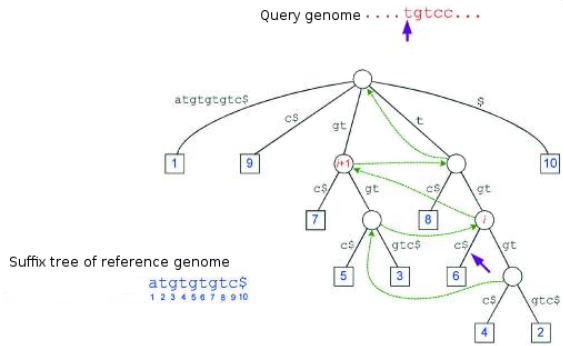
\includegraphics[scale=0.8]{st-mum.png} 
   \caption{Árbol de sufijos para la palabra atgtgtgtc\$.} 
   \label{fig:st} 
 \end{figure}
\indent
La búsqueda de coincidencias exactas máximas en un árbol de sufijos se realiza recorriendo el árbol
con la cadena que se requiere encontrar la coincidencia exacta máxima. Si la coincidencia termina en 
un nodo hoja, la coincidencia exacta máxima es única en la secuencia de referencia. Verificando el 
carácter inmediato anterior al inicio de la posición de la coincidencia es posible determinar si es
máxima.\\
\indent
Por lo tanto es posible identificar todas las coincidencias exactas máximas en tiempo proporcional a
la longitud del genoma de consulta. Es importante resaltar que las coincidencias encontradas no son
necesariamente únicas en el genoma de consulta. Esto se debe a que al recorrer el genoma de consulta, 
las coincidencias encontradas no nos permiten identificar si son únicas ya que no es posible determinar
que coincidencias se encontrarán posteriormente en el genoma de consulta.\\
\indent
En la Figura \ref{fig:st} se muestra como una secuencia de consulta es buscada en el árbol de sufijos. El
árbol representa la secuencia de referencia atgtgtgtc\$. Las hojas representadas por cuadrados indican la
posición en la que inicia el sufijo. Por ejemplo, la hoja 7 representa el sufijo gtc\$ que inicia en la 
posición 7 de la secuencia de referencia y que está formado por la secuencia de aristas etiquetadas desde la
raíz hasta el nodo hoja 7. En el punto mostrado en la figura, se ha encontrado la coincidencia en la posición $i$,
indicada por la flecha. La coincidencia se extiende a la correspondiente posición en el árbol. En este caso sabemos
que la coincidencia es única en la referencia por que estamos ubicados en un nodo hoja. El número del nodo hoja
nos da la posición de inicio de la coincidencia en la referencia.\\
\indent
Para encontrar la siguiente coincidencia, usamos los enlaces de sufijos, señalados en la Figura \ref{fig:st} por
flechas punteadas. Estos enlaces son construidos para cada nodo interno en el árbol. Un enlace apunta de un nodo
$x$ a un nodo $y$ si el sufijo de la raíz a $y$ es igual al sufijo desde la raíz a $x$ con el primer carácter 
eliminado. Por ejemplo, la cadena del nodo $i$ en la Figura \ref{fig:st} es tgt y del nodo $i+1$ es gt. Esa es la
posición en el árbol correspondiente a la siguiente posición en la secuencia de consulta. Desde el nodo $i$ podemos
continuar la coincidencia bajando en el árbol para determinar que tan grande es la coincidencia puede extenderse. Las 
coincidencias son máximas hacia la derecha cuando se buscan en el árbol de sufijos. Para verificar si son máximas a
la izquierda comparamos los caracteres precedentes en cada cadena. En el ejemplo de la Figura \ref{fig:st}, la
coincidencia inicia en $i+1$ en la cadena de consulta y en el nodo 7 de la cadena del árbol no es máxima a la izquierda
porque el carácter precedente en ambas cadenas es $t$.\\
\indent
El primer algoritmo para la construcción de un árbol de sufijos en tiempo lineal 
y eficiente en espacio fue propuesto en \cite{McCreight:1976:SST:321941.321946}
, y Ukkonen produjo una variante ``on-line'' de ese algoritmo en \cite{Ukkonen1992}. 
La clave para la búsqueda veloz en un árbol de sufijos es que 
hay un camino desde la raíz para cada sufijo del texto. Esto significa que se 
necesitan $l$ comparaciones para encontrar una cadena de longitud $l$.\\
\indent
Otra mejora de implementación necesario para conseguir un tiempo y espacio 
lineal es el uso de enlaces de sufijos. Un enlace de sufijo es un puntero de un 
nodo interno etiquetado $xS$ a otro nodo interno etiquetado $S$, donde $x$ es un 
carácter arbitrario y $S$ es posiblemente una subcadena vacía. Los enlaces de 
sufijos permiten agilizar el recorrido del árbol sin visitar la raíz del árbol 
debido a que apuntan a la siguiente extensión del sufijo. Los enlaces de sufijos 
y la compresión de las etiquetas de las aristas son los requerimientos claves 
para la implementación del árbol de sufijos en $O(n)$.\\
\indent
Existen diferentes implementaciones de árboles de sufijos, cada uno con 
complejidades espaciales diferentes como se muestra en el Cuadro \ref{tab:stmem}.\\
\begin{table}[h!]  
\begin{small}
\begin{center}
\begin{tabular}{lll}
Algoritmo & Complejidad espacial & Tamaño \\
\hline
McCreight & $O(28n)$ & 81.48GB \\
\hline
Ukkonen & $O(26.4n)$ & 76.95GB \\
\hline
Kurtz & $O(15.5n)$ & 45.31GB \\
\hline
Sadakane\footnote{Compresión de árbol de sufijos} & $O(n\log|\Sigma|)$ & 8.8GB \\
\hline
TRELLIS \cite{Phoophakdee2007} & $O(24.6n)$ & 71.6GB \\
\hline
TDD \cite{Barsky2010} & $O(18.5n)$ & 54GB \\
\end{tabular}
\end{center}
\end{small}
\caption{Algoritmos de creación de árboles de sufijos y su uso de memoria al
almacenar el genoma humano (n=2.91Gbp).}
\label{tab:stmem}
\end{table}
\\ \indent
Los árboles de sufijos son dependientes del alfabeto, $\Sigma$, el tamaño 
del alfabeto, $|\Sigma|$, afecta los tiempos de creación y búsqueda de 
cadenas en el árbol, $C$, para una cadena de referencia de longitud $n$. 
Estrictamente hablando:
    \begin{itemize} 
      \item Requerimiento de espacio: $O(n)$ 
      \item Tiempo de creación: $min (O(n\log n), O(n\log |\Sigma|))$ 
      \item Tiempo de búsqueda: $min (O(|C|\log n), O(|C|\log |\Sigma|))$ 
    \end{itemize}
\indent
\subsection{Definición del problema a resolver}
\indent
El problema de la búsqueda de las coincidencias exactas máximas de una longitud mínima han sido identificados en varias aplicaciones, entre ellas MUMmer \cite{Mummer3}. Aunque el algoritmo de MUMmer realiza la búsqueda de coincidencias exactas máximas, los requerimientos de recursos de cómputo aún son altos debido al tamaño de los datos de entrada.\\
\indent
Se ha realizado un experimento para comparar las prestaciones de la búsqueda de
coincidencias exactas máximas utilizando un árbol de sufijos. En el Cuadro 
\ref{tab:buscar} se muestra el tiempo de procesamiento de búsqueda 
para coincidencias de tamaño mínimo $L$, utilizando el árbol de sufijos. El tiempo 
de cómputo invertido en la búsqueda involucra la operación individual de cadenas de longitud mínima $L$ hasta la longitud de la cadena máxima de coincidencia. \\
\begin{table}[ h!] 
  \begin{small}
    \begin{center}
      \begin{tabular}{lllll}
        Estructura & L [bp] & Cantidad  & Búsqueda [s] & Uso de\\
        & & de búsquedas & & memoria [MB] \\
        \hline
        Árbol de sufijos & 20 & 344,46\e{6}  & 1679,2 & 483 \\
        %\hline
        %Arreglo de sufijos & 20 & 344,46\e{6}  & 5885,7 & 320\\
        \hline
      \end{tabular}
    \end{center}
  \end{small}
  \caption{Búsqueda coincidencias exactas para una cadena de referencia de 
  29,38Mbp y una cadena de consulta de 29,69Mbp}
  \label{tab:buscar}
\end{table}
\indent
El tiempo de búsqueda del Cuadro \ref{tab:buscar} para cadenas de tamaño de 30Mbp
es relativamente alto debido a que involucra realizar millones de búsquedas en
serie. La cantidad de operaciones de búsqueda que se realizan son 11 veces la 
longitud de las cadenas de referencia y consulta. En consecuencia, la búsqueda 
de coincidencias exactas máximas es una operación computacionalmente intensiva. 
La razón de este uso intensivo de cómputo se debe a la cantidad de operaciones de búsqueda
y a los accesos aleatorios en memoria al hacer cada operación de búsqueda.\\
\indent
Al aumentar la longitud de las cadenas de referencia y consulta por un factor de 10, 
los tiempos de búsqueda se incrementan linealmente por un factor de 10, el uso de 
memoria aumenta aproximadamente 8 veces y la cantidad de búsquedas a realizar se
multiplica \e{3} veces, como se observa en el Cuadro \ref{tab:buscar2}.\\
\begin{table}[ h! ]
  \begin{small}
    \begin{center}
      \begin{tabular}{lllll}
        Estructura & L [bp] & Cantidad  & Búsqueda [s] & Uso de\\
        & & de búsquedas & & memoria [MB] \\
        \hline
        Árbol de sufijos & 20 & 3,78\e{9}  & 13013,5 & 3890 \\
        %\hline
        %Arreglo de sufijos & 20 & 3,78\e{9}  & 45616,2 & 2293\\
        \hline
      \end{tabular}
    \end{center}
  \end{small}
  \caption{Búsqueda coincidencias exactas para una cadena de referencia de 
  227,69Mbp y una cadena de consulta de 238,62Mbp}
  \label{tab:buscar2}
\end{table} 
\indent
Si la longitud de las cadenas crece por un factor de 10, ver Cuadro \ref{tab:buscar3}, 
la cantidad de búsquedas son aproximadamente \e{18}, el tiempo de búsqueda
crece linealmente y el uso de memoria se convierte en un problema a analizar si
se considera la disponibilidad finita de memoria en la mayoría de sistemas de
cómputo personales.\\
\begin{table}[ h!]
  \begin{small}
    \begin{center}
      \begin{tabular}{lllll}
        Estructura & L [bp] & Cantidad  & Búsqueda [s] & Uso de\\
        & & de búsquedas & & memoria [MB]\\
        \hline
        Árbol de sufijos & 20 & 9,87\e{18}  & 169189,4 & 48665,12\\
        \hline
        %Arreglo de sufijos & 20 & 9,87\e{18}  & 593019,3 & 32241,9\\
        %\hline
      \end{tabular}
    \end{center}
  \end{small}
  \caption{Búsqueda coincidencias exactas para una cadena de referencia de 
  2960,21Mbp y una cadena de consulta de 2716,96Mbp}
  \label{tab:buscar3}
\end{table}
\indent
De acuerdo a los datos de los Cuadros \ref{tab:buscar}, \ref{tab:buscar2} y 
\ref{tab:buscar3} se hace necesario la búsqueda de alternativas que 
permitan llevar a cabo la búsqueda de manera eficiente. El uso de HPC nos permitiría
resolver los problemas de escalabilidad (tiempo de búsqueda, uso de memoria) cuando 
se tienen cadenas muy grandes, como el genoma humano.\\
\subsection*{Problema} 
\indent
La búsqueda de coincidencias exactas máximas es un problema computacionalmente
intensivo. Dadas una cadena de referencia $R$ de longitud $n$ y una cadena de consulta 
$Q$ de longitud $m$, encontrar todas las coincidencias de longitud mínima $l$ de $Q$
en la cadena de referencia $R$ implica recorrer la cadena de consulta $Q$ para $todas$
sus subcadenas. Para cada subcadena se determina la posición o posiciones en donde 
existe una coincidencia, de longitud mínima $l$, entre la subcadena y la cadena de 
referencia $R$. La posición de la subcadena en $Q$ es determinada.\\
\indent
En la Figura \ref{fig:problema} se muestra gráficamente el problema de la búsqueda
de coincidencias exactas máximas.
\begin{figure}[h]
\begin{center}
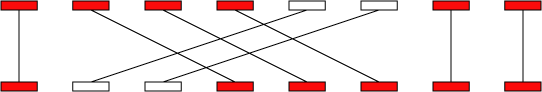
\includegraphics[scale=0.5]{gaps.png}
\caption{Problema de la búsqueda de coincidencias exactas máximas.}
\label{fig:problema}
\end{center}
\end{figure}
\\ \indent El total de búsquedas, indicado en los Cuadros \ref{tab:buscar} y \ref{tab:buscar2} 
a realizar está determinada por la fórmula \ref{eq:operaciones}.
\begin{equation}
  \sum_{i=0}^{i\le m}{\frac{n}{L+i}}
  \label{eq:operaciones}
\end{equation}
Realizar una búsqueda de coincidencia exacta de longitud fija es sencilla 
computacionalmente hablando. Pero al realizar una búsqueda de coincidencia exacta de 
longitud variable ocurren los siguientes problemas:
\begin{itemize}
  \item Acceso aleatorio a la cadena indexada de referencia $R$: el conjunto de coincidencias
    podría estar en posiciones de la cadena $R$ distantes.
  \item Longitud variable de la cadena a buscar: la búsqueda a realizar se incrementa
    con la longitud de la cadena.
  \item Uso de memoria: para poder buscar una coincidencia se requiere volcar la 
    cadena de referencia $R$ en memoria. Dependiendo del método utilizado la 
    cantidad de memoria se podría incrementar e incluso agotar la memoria disponible.
    Adicionalmente el tiempo de búsqueda se incrementará, como se observa en el 
    Cuadro \ref{tab:buscar3},debido al acceso a disco cuando no se tiene toda la 
    cantidad de memoria necesaria.
\end{itemize}
Para resolver este problema de forma distribuida existen diferentes estrategias. La 
solución mas obvia es realizar una división de las cadenas de referencia y
de consulta, ver Figura \ref{fig:para}.
\begin{figure}[h]
\begin{center}
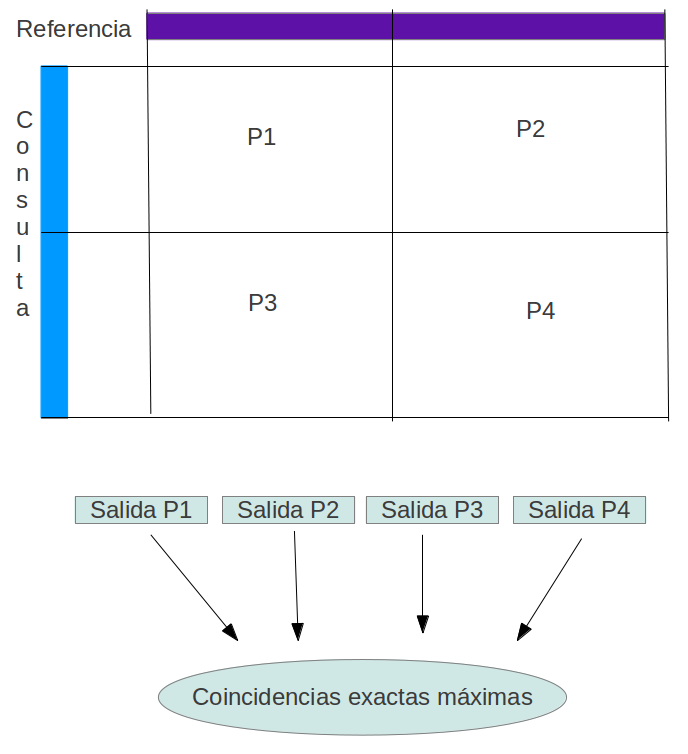
\includegraphics[scale=0.3]{naive.png}
\caption{Solución obvia de paralelización de búsqueda de coincidencias exactas máximas.}
\label{fig:para}
\end{center}
\end{figure}
\\Esta técnica ocasiona que exista una fase de procesamiento posterior a la búsqueda de 
coincidencias exactas máximas en cada segmento de la cadena procesada, para determinar
las coincidencias máximas de forma global. Adicionalmente, puede haber pérdidas de 
coincidencias máximas exactas y coincidencias máximas que solo son válidas dentro del 
segmento evaluado y no de manera global.\\
En consecuencia, para resolver este problema se utiliza alguna estructura de datos que 
permita realizar una búsqueda distribuida de coincidencias exactas máximas de forma ágil 
en la cadena entera. Los árboles de sufijos permiten hacer 
búsquedas con complejidad $O(m+k)$, donde $m$ es el 
tamaño de la cadena a buscar y $k$ es el número de ocurrencias.\\
En resumen la búsqueda de coincidencias exactas máximas en una cadena, como el 
genoma humano, es un problema computacionalmente intensivo que es posible 
resolverse con estructuras de datos como el árbol de sufijos. 
%Sin embargo como se 
%muestra en el Cuadro \ref{tab:estructuras} se reseña las características de cada solución propuesta.\\
%\begin{table}[hc]   
%\begin{small}
%\begin{center}
%\begin{tabular}{llllll}
%Estructura de datos & Memoria & Búsqueda & Ventaja & Desventaja\\
%\hline
%Arreglo de sufijos & $O(10n)$  & $O(m\log n)$, & Eficiente en & Tiempo de búsqueda 
%en  \\ 
%& & $m$ es el tamaño de & uso de espacio.& de coincidencias exactas \\
%& & la cadena a buscar.& inaceptable.\\
%\hline
%Árbol de sufijos & $O(15.5n)$ & $O(m+k)$, & Búsqueda de   & Incremento en \\
%&  &  $m$ es el tamaño de & de coincidencia de & el tiempo de \\ 
%&  & la cadena buscar & cadenas de & búsqueda. \\
%&  &y $k$ el número de ocurrencias. & longitud variable.&\\
%\end{tabular}
%\end{center}
%\end{small}
%\caption{Estructuras de datos para la búsqueda de coincidencia exacta de cadenas.}
%\label{tab:estructuras}
%\end{table}
\\Independientemente de la estructura de datos utilizada, lo que se desea es poder
realizar búsquedas de coincidencias exactas a esa estructura de manera eficiente. 
Una de las consultas en que se requiere realizar rápidamente, para el alineamiento 
de genomas, es la búsqueda exacta de coincidencias máximas. 
\section{Estado de la investigación}
\subsection{Búsqueda distribuida de coincidencias exactas: árbol de sufijos distribuido}
El problema de mejorar el tiempo de cómputo de las búsquedas de coincidencias 
exactas nos da una oportunidad de utilizar el poder del HPC para reducir el
tiempo de procesamiento. Se propone modificar la estructura de datos utilizada en 
MUMmer (árbol de sufijos) para mejorar las búsquedas de coincidencias exactas en 
grandes volúmenes de datos, considerando un uso eficiente de los recursos. Para 
ello se tomarán en cuenta los siguientes parámetros: 
\begin{itemize}
\item Tamaño del genoma de referencia y consulta.
\item Memoria principal disponible en cada nodo de cómputo.
%\item Búsqueda distribuida de coincidencias exactas.
\end{itemize}
Basado en dichos parámetros se distribuirá el árbol de sufijos en subárboles, 
ver Figura \ref{fig:estructura}. Dicha aproximación ha sido llevada a cabo de distintas maneras por \cite{Mansour2012}, 
\cite{Japp2004}, \cite{Ghoting2010} y \cite{Sadakane}.
 Los subárboles aprovecharán una característica
de la búsqueda de coincidencias: el acceso frecuente a la parte superior del 
árbol de sufijos.\\ 
\begin{figure}[h]
\begin{center}
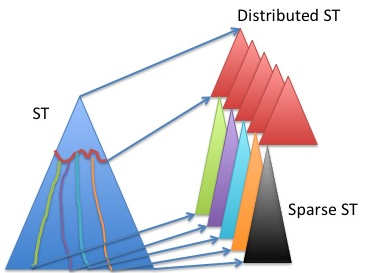
\includegraphics[scale=0.8]{distributed.png}
\caption{Árbol de sufijos distribuido.}
\label{fig:estructura}
\end{center}
\end{figure}
Para definir formalmente el árbol de sufijos distribuido es necesario definir 
algunos conceptos, extraídos de \cite{Clifford2005} y \cite{Ghoting2010}. 
\begin{mydef}
  Si $t=uvw$ entonces $u$ es un \textit{prefijo} y $w$ es un \textit{sufijo}
de $t$.
\end{mydef}
Un sufijo de $t$ se repite si ocurre al menos una vez como una subcadena no sufijo de $t$.
Además requerimos poder especificar que sufijos de $t$ se incluyen en un subárbol de sufijos. Esto
se hace considerando un prefijo corto $z$, y un conjunto de posiciones iniciales, $V_{z}$.
\begin{mydef}
  Para aquellos sufijos de la referencia que tienen la cadena $z$ como un prefijo.$V_{z}$ es el conjunto válido.
\end{mydef}
\begin{mydef}
Una subcadena $s$ de $t$ es válida si $z$ es un prefijo de $s$ y que un intervalo de enteros $I[i,j]$ es
\textit{válido} (con respecto a $V_{z}$ y $t$) si $i$ $\epsilon$ $V_{z}$.
\end{mydef}
\begin{mydef}
  $s$ es un \textit{sufijo válido} para $I[i,j]$ si $s=t[k,j]$ para algún $k$ $\epsilon$ $V_{z}$ y $k>i$. 
\end{mydef}
Es posible que un sufijo válido para un intervalo puede ser mas corto que el prefijo fijo $z$, dependiendo de 
los caracteres que siguen directamente en la referencia.\\
\begin{mydef}
  Sea $z$ una cadena de longitud mayor o igual a 1. Decimos que $(t,V_{z})$ es un \textit{par de entrada} si $V_{z}$ es
el conjunto válido (para $t$ con respecto a $z$).
\end{mydef}
Escribimos $sst(t,V_{z})$ para el árbol de sufijos poco denso de $t$ usando el conjunto válido $V_{z}$. 
\begin{mydef}
  Para un árbol de sufijos poco denso $T=sst(t,V_{z})$ y un conjunto arbitrario de cadenas $S$, decimos que
  $T'=T aumentado$ por $S$ si $T'$ es una trie compactada de la unión de $S$ y el conjunto sufijos válidos de
  $t$ (con respecto a $V_{z}$).
\end{mydef}
Para construir el árbol de sufijos distribuido DST en tiempo lineal se construye un SST en tiempo lineal
y se ejecuta el algoritmo de construcción del árbol para diferentes prefijos escogidos. El algoritmo
resultante usa el espacio en cada nodo que es proporcional al tamaño del SST construido.
\subsection{Importancia del enlace de sufijo}
Los enlaces de sufijos juegan un rol crítico en la construcción lineal de árboles de sufijos y en su
recorrido.
\begin{mydef}
  Si hay un nodo v en el árbol de sufijos con la etiqueta $c\alpha$, donde c es un carácter y $alpha$
  es una cadena (no vacía), entonces el enlace de sufijo de v apunta a s(v), que es un nodo con la
  etiqueta $\alpha$. Si $\alpha$ está vacío, entonces el enlace de sufijo de v, por ejemplo s(v) es la
  raíz. 
\end{mydef}
Los enlaces de sufijo existen para cada nodo interno (no hoja) de un árbol de sufijo. Siguiendo un 
enlace de sufijo, se puede saltar de un sufijo a otro, cada sufijo iniciando exactamente un carácter
siguiente del primer carácter de su sufijo precedente. De tal manera que usando enlaces de sufijos es
posible obtener un algoritmo lineal para la búsqueda de coincidencias exactas máximas. Esto es porque
los enlaces de sufijos hacen un seguimiento de que o cuanto de la cadena ha coincidido hasta ahora.
Cuando encontramos una falta de coincidencia, podemos saltar a lo largo del enlace de sufijo para 
ver si hay cualquier coincidencia despu\'es en la referencia y en la consulta.
\begin{mydef}
  Considerar un par de entrada $(t,V_{z})$ y un árbol de sufijos poco denso $T=sst(t,V_{z})$. Un enlace
  de sufijo disperso es un borde sin etiquetar de $\overline{aw}$ a la raíz si $|v|<|z|$ y de $\overline{aw}$
  a $\overline{v}$, de otra manera.
\end{mydef}
Mediante la organización del nuevo árbol de sufijos distribuido de esta manera, 
podemos realizar búsquedas de coincidencias exactas máximas de forma distribuida. Al
utilizar una búsqueda distribuida es posible mejorar el tiempo de cómputo de 
las búsquedas exactas. Se requiere que el tiempo de cómputo sea menor que el 
mostrado por propuestas existentes en el estado del arte y que pueda manejar
genomas de gran tamaño.\\
\subsection{Evaluación experimental}
Para determinar el par de entrada $(t,V_{z})$ es necesario determinar el acceso a los prefijos dentro del
árbol de sufijos. Es por ello que se realizó un experimento para ubicar la longitud necesaria para la 
elección de los prefijos. En la siguiente figura \ref{fig:top} se muestra en la zona azul la parte superior
del árbol de sufijos y las líneas rojas muestran el pintado del árbol para indicar la ubicación de una 
coincidencia máxima en el árbol.Para determinar el par de entrada $(t,V_{z})$ es necesario determinar el acceso a los prefijos dentro del
árbol de sufijos. Es por ello que se realizó un experimento para ubicar la longitud necesaria para la 
elección de los prefijos. 
\begin{figure}[h]
\begin{center}
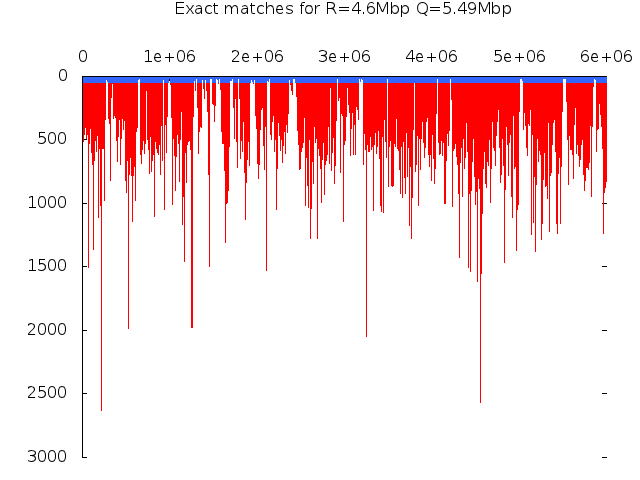
\includegraphics[scale=0.4]{freq.png}
\caption{Identificación de coincidencias máximas en árbol de sufijos.}
\label{fig:top}
\end{center}
\end{figure}
Este experimento nos permite confirmar que la ubicación de cada uno de los prefijos difiere en longitud, debido a 
esto se hace necesario definir prefijos de longitud variable. Al utilizar prefijos de longitud variable es posible
tener árboles de sufijos dispersos balanceados debido a que se podrían agrupar aquellos prefijos con mayor frecuencia
de ocurrencia.\\
Es por ello que debemos encontrar un conjunto valido de prefijos para dividir el árbol de sufijos en árboles de sufijos
dispersos con el requerimiento de que puedan construirse en memoria principal.
\begin{mydef}
Sea $f(p)$ el número de veces que un prefijo ocurre en S. Sea MSSTS (tamaño máximo del árbol de sufijos disperso) la cantidad
máxima de espacio de memoria en bytes que puede ser reservado al árbol de sufijos disperso durante la construcción del árbol. 
Sea NS el tamaño de un nodo del árbol de sufijos en bytes.
\end{mydef}
El objetivo es encontrar un conjunto de pares de entrada valido tal que $\forall p \epsilon V_{z}, 2xf(p)<\frac{MSSTS}{NS}$.\\
Una vez definido el conjunto de prefijos se procede a la construcción del árbol de sufijos disperso. Para ello se ubican en cada
árbol de sufijos disperso el conjunto de pares de entrada valido que serán las raíces de cada árbol de sufijos disperso. Una vez 
definido el conjunto de prefijos se procede a la construcción del árbol de sufijos disperso.\\
La construcción del árbol de sufijos disperso se realiza siguiendo el algoritmo de Ukkonen y removiendo aquellos nodos y bordes
que no tienen en común el prefijo de la raíz del árbol de sufijo disperso.\\
En la figura \ref{fig:dst} se muestra el árbol de sufijos distribuido con cada uno de los árboles de sufijos disperso. Para una
cadena aacacccacacaccacaaa\$ con sus respectivos nodos raíz etiquetados como $r_{aa}, r_{ac}, r_{ca}, r_{cc}, r_{a\$}$ and $r_{\$}$.
\begin{figure}[h]
\begin{center}
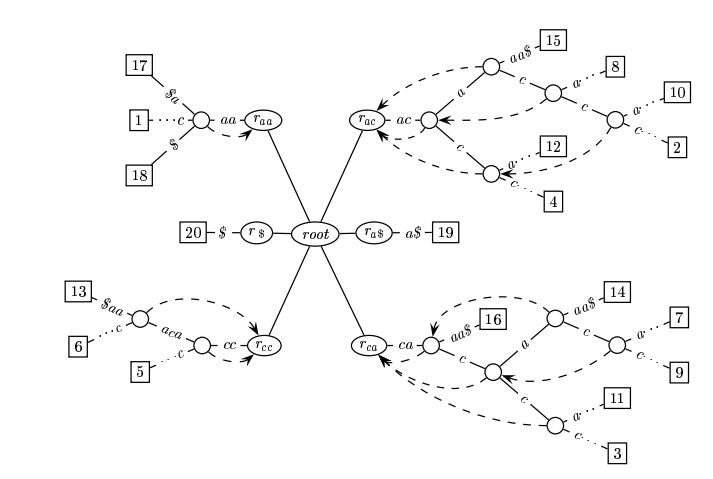
\includegraphics[scale=0.4]{dst2.png}
\caption{Árbol de sufijos distribuido para la cadena: aacacccacacaccacaaa\$.}
\label{fig:dst}
\end{center}
\end{figure}
Una característica que el árbol de sufijos distribuido tiene es que únicamente mantiene los enlaces de sufijos que pertenecen al 
árbol de sufijos disperso. Aquellos enlaces de sufijos que apunten a otros nodos que no están en el árbol de sufijos disperso
son descartados en la fase de construcción del árbol.\\
Como se mencionó anteriormente el enlace de sufijo no solo permite la construcción en tiempo lineal del árbol de sufijos sino
que hace que las búsquedas de coincidencias sean tambi\'en lineales. En consecuencia surge ahora un nuevo problema al proponer
esta estructura de datos modificada:\\
\begin{center}
  ¿Es posible mantener la complejidad de búsqueda de coincidencias en un árbol de sufijos $O(m+k)$, en donde $m$ es la
  longitud de la secuencia de consulta y $k$ es el número de ocurrencias al utilizar un árbol de sufijos distribuido?
\end{center}
Para determinar el impacto del uso de los enlaces de sufijos en un árbol de sufijos se ejecutaron algunos experimentos para
conocer la utilización de los enlaces de sufijos al hacer la búsqueda de coincidencias y la ubicación de los enlaces de sufijos
dentro del árbol de sufijos.\\
En las figuras \ref{fig:st_sl} y \ref{fig:st_sl2} se muestra el recorrido del árbol de sufijos. Para cada uno de los sufijos
de la secuencia de consulta al utilizar el enlace de sufijo se avanza en el árbol de sufijos hacia arriba o abajo. Al navegar
con el enlace de sufijo se evita hacer comparaciones de acuerdo a la ubicación del nodo dentro del árbol de sufijos, es decir,
se consumen $x$ caracteres.
\begin{figure}[h]
\begin{center}
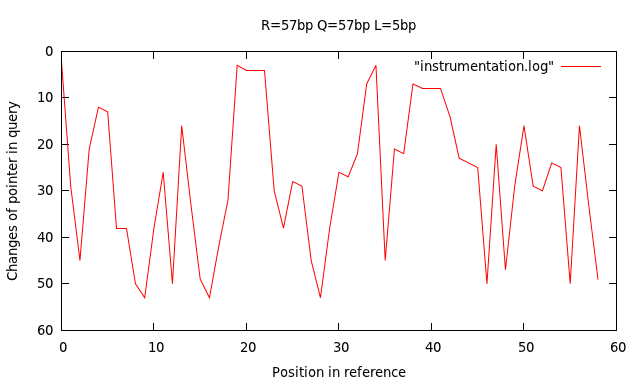
\includegraphics[scale=0.4]{r57-q57-l5.png}
\caption{Recorrido del árbol de sufijos al utilizar los enlaces de sufijos.}
\label{fig:st_sl}
\end{center}
\end{figure}
\begin{figure}[h]
\begin{center}
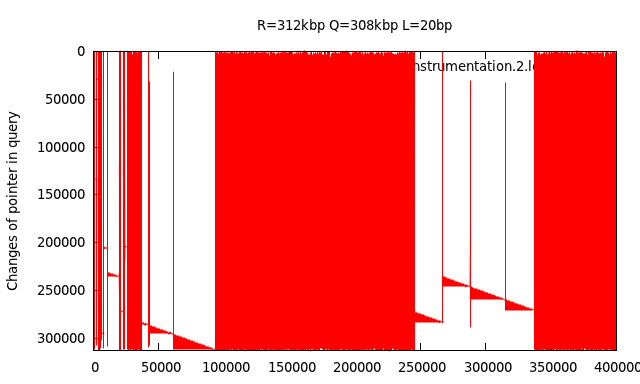
\includegraphics[scale=0.4]{r312kbp-q308kbp-l20.png}
\caption{Recorrido del árbol de sufijos al utilizar los enlaces de sufijos.}
\label{fig:st_sl2}
\end{center}
\end{figure} 
Una vez definido la utilización de los enlaces de sufijos se procede a determinar en que posiciones dentro del árbol de sufijos
se ubican los enlaces de sufijos. Para ello se realizó un conteo del número de enlaces de sufijos. En las figuras \ref{fig:hist_sl}
y \ref{fig:hist_sl2}. Esta evaluación nos permite identificar que el uso de los enlaces de sufijos es dependiente de la secuencia
de referencia y que la mayoría de los enlaces de sufijos se encuentran en la zona inferior del árbol de sufijos.
\begin{figure}[h]
\begin{center}
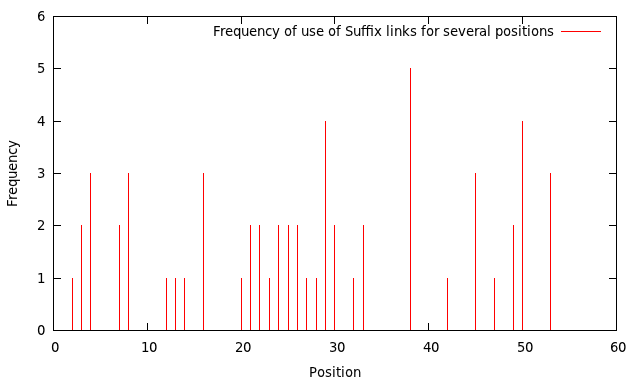
\includegraphics[scale=0.4]{histogram2.png}
\caption{Frecuencia de enlaces de sufijos.}
\label{fig:hist_sl}
\end{center}
\end{figure}
\begin{figure}[h] 
\begin{center}
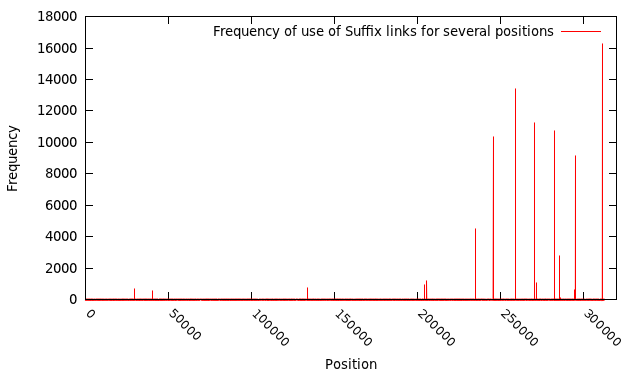
\includegraphics[scale=0.4]{histogram.png}
\caption{Frecuencia de enlaces de sufijos.}
\label{fig:hist_sl2}
\end{center}
\end{figure}
\subsection{Búsqueda de coincidencias exactas en un DST}
El propósito de adaptar una estructura de datos como el árbol de sufijos es lograr reducir el tiempo de búsqueda de coincidencias
exactas. Para ello se propone una primera aproximación a la búsqueda de coincidencias exactas máximas en un árbol de sufijos 
distribuido.\\
La idea general se basa en dividir la secuencia de consulta en segmentos y asignar la búsqueda de cada sufijo dentro de cada
segmento en el árbol de sufijos disperso correspondiente. La búsqueda de coincidencias exactas sigue en el árbol de sufijos y 
posteriormente determina las posiciones en las cuales se encuentran las coincidencias. Al evaluar el siguiente sufijo pueden
ocurrir dos casos:
\begin{enumerate}
  \item El siguiente sufijo se encuentra en el mismo árbol de sufijos disperso. La búsqueda continúa de manera local.
  \item La búsqueda del siguiente sufijo se realiza en otro árbol de sufijos disperso.
\end{enumerate}
El segundo caso es de especial relevancia ya que implica el proponer una estrategia de búsqueda del árbol de sufijos disperso
en donde se debe realizar la búsqueda y adicionalmente continuar la búsqueda en ese árbol.\\
Para solucionar este caso, se propone el envío de la petición de búsqueda del sufijo en el árbol correspondiente. Para determinar
el árbol de sufijos disperso que le corresponde el árbol consulta el prefijo del sufijo y envía la ubicación del sufijo al árbol 
de sufijos disperso correspondiente. El árbol que recibe la petición la encola en la lista de sufijos que tiene que procesar y 
resuelve la búsqueda de coincidencias exactas máximas del sufijo que se le ha asignado.\\
En la figura \ref{fig:dst_search} se muestra de manera gráfica la búsqueda de coincidencias exactas para una secuencia de consulta,
la división en segmentos de la misma y la búsqueda del primer sufijo de cada segmento en el árbol de sufijos distribuido.
\begin{figure}[h] 
\begin{center}
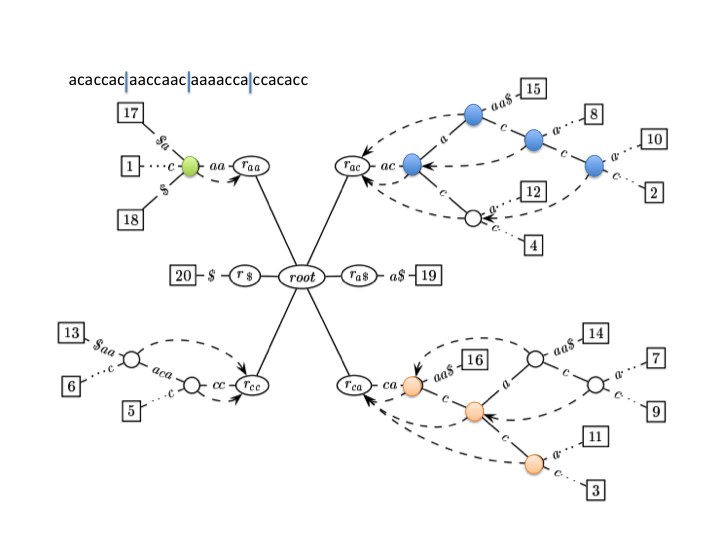
\includegraphics[scale=0.4]{dst_search.png}
\caption{Búsqueda de coincidencias exactas máximas en un árbol de sufijos distribuido.}
\label{fig:dst_search}
\end{center}
\end{figure}

\section{Publicaciones}
\noindent
Ninguna.
\section{Seguimiento}
En el primer año se ha cumplido con la adaptación de una estructura de datos que permita su utilización
en el alineamiento de datos biológicos a gran escala. Dicha estructura será la base del desarrollo de MUMmer en HPC.
La estructura es capaz de manejar grandes volúmenes de datos y se pueden realizar operaciones de consulta sobre ella.
\section{Planificación}
En el segundo año se realizará el diseño y evaluación experimental de un algoritmo paralelo y distribuido de búsquedas de 
coincidencias exactas máximas. Para ello se aprovechará la estructura de datos diseñada en el primer año. Se adaptará este
algoritmo a la aplicación MUMmer para su ejecución en entornos de HPC.
En el tercer año se refinará la ejecución de MUMmer en entornos de HPC. Se tomará como base el programa original, MUMmer, y 
se realizarán las modificaciones pertinentes para mejorar la fase de agrupamientos de MUMs y MEMs. Estancia en otra unidad 
de investigación, EMBL Heidelberg Alemania. Adaptar la propuesta de búsqueda distribuida de coincidencias exactas desarrollado para su
ejecución en las instalaciones de EMBL. Redactar la tesis doctoral y preparar su defensa.
\section{Análisis de las publicaciones pendientes de publicar}
\noindent
Ninguna.
\section{Publicaciones previstas}
European Symposium on Algorithms - \href{http://esa-symposium.org/}{ESA} - Abril 2013\\
International Symposium on Algorithms and Computation - \href{http://www.is.titech.ac.jp/isaac11/}{ISAAC} - 2013\\
International Conference on Parallel Processing - \href{http://www.grs-sim.de/news-events/news-archive/euro-par-2013.html}{Euro-Par} - 2013\\
Asia Pacific Bioinformatics Conference - \href{http://www.bioinformatics.ubc.ca/2012/01/30/apbc2013-the-eleventh-asia-pacific-bioinformatics-conference/}{APBC} - Julio 2012\\
IEEE International Symposium on Parallel and Distributed Processing with Applications - \href{http://www.arcos.inf.uc3m.es/ispa12/}{ISPA} - 2013

\section{Conclusiones}
\indent
Durante este primer año de investigación doctoral se ha estudiado y evaluado la estructura de datos utilizada en la aplicación MUMMer.
Se han diseñado diferentes experimentos para determinar la mejor manera de dividir dicha estructura y aprovechar la nueva estructura
en entornos de HPC. Se evalúo la utilidad de los enlaces de sufijos en un árbol de sufijos y como se pueden aprovechar para la 
búsqueda de coincidencias exactas máximas.\\
\indent
Se ha adaptado el árbol de sufijos para su ejecución en entornos de HPC y se ha propuesto una solución al problema de  la restricción
de memoria cuando la cadena de referencia crece. La estructura de datos adaptada se ha utilizado para proponer una primera aproximación a la 
solución de mejorar el tiempo de búsqueda de coincidencias exactas máximas.\\
\indent
En el siguiente año se busca determinar si la propuesta de búsqueda de coincidencias exactas máximas en el árbol de sufijos distribuido 
permite mejorar el tiempo de ejecución bajo entornos de HPC. Adicionalmente se tendrán que resolver los siguientes problemas
\begin{itemize}
  \item Política de carga de trabajo para cada árbol de sufijos disperso: garantizar que todas las búsquedas se resuelvan de manera local.
  \item Búsqueda de coincidencias exactas máximas en el árbol de sufijos disperso de forma paralela, es decir, realizar múltiples búsquedas
    para distintos sufijos. 
\end{itemize}
\bibliographystyle{apalike} 
\bibliography{references}	
\end{document}
